
\serie{Produits de relatifs}

\begin{exercice}
Complète : 
\begin{enumerate}
 \item $A = (-4) + (-4) + (-4) + (-4) + (-4)$
 
$A = (-4) \times \ldots \ldots$

$A = \ldots \ldots$
 \item $B = (-8,2) + (-8,2) + (-8,2)$
 
$B = (-8,2) \times \ldots \ldots$

$B = \ldots \ldots$
 \item $C = (-1,7) + (-1,7) + (-1,7) + (-1,7)$

$C = (-1,7) \times \ldots \ldots$

$C = \ldots \ldots$
 \end{enumerate}
\end{exercice}


\begin{exercice}
Sans les calculer, donne le signe de chacun des produits suivants :
\begin{colenumerate}{2}
 \item $(-12) \times (+2)$ \dotfill;
 \item $(+34) \times (-28)$ \dotfill;
 \item $(-10,3) \times (-46)$ \dotfill;
 \item $(+12,5) \times (+3,1)$\dotfill.
 \end{colenumerate}
\end{exercice}


\begin{exercice}
Sans les calculer, donne le signe de chacun des produits suivants :
\begin{colenumerate}{2}
 \item $-36 \times (-1)$ \dotfill;
 \item $(-2) \times (+24)$ \dotfill; 
 \item $2,3 \times (-2,3)$ \dotfill;
 \item $-9,1 \times 6$\dotfill.
 \end{colenumerate}
\end{exercice}


\begin{exercice}
Quel est le signe du résultat quand on :
\begin{enumerate}
 \item multiplie un nombre négatif par un nombre positif ? \ldots \ldots
 \item multiplie quatre nombres négatifs entre eux ?  \ldots \ldots
 \item multiplie un nombre positif et deux nombres négatifs ?  \ldots \ldots
 \item multiplie un nombre relatif par lui-même ? \ldots \ldots
 \item multiplie trois nombres négatifs entre eux ? \ldots \ldots
 \end{enumerate}
\end{exercice}


\begin{exercice}
Effectue :
\begin{colenumerate}{2}
 \item $(+5) \times (-4)$ \dotfill;
 \item $(-5) \times (-3)$ \dotfill;
 \item $(-3) \times (+4)$ \dotfill;
 \item $(+4) \times (+4)$ \dotfill;
 \item $(-4) \times (-3)$ \dotfill;
 \item $(-5) \times (-4)$ \dotfill;
 \item $(-5) \times (+3)$ \dotfill;
 \item $(-4) \times (+4)$\dotfill.
 \end{colenumerate}
\end{exercice}


\begin{exercice}
Effectue :
\begin{colenumerate}{2}
 \item $(-8) \times (+2)$ \dotfill;
 \item $(-2) \times (+5) $ \dotfill;
 \item $(-4) \times (-8)$ \dotfill;
 \item $(+9) \times (+10)$ \dotfill; 
 \item $(+191) \times (+0,1)$ \dotfill; 
 \item $(-1,5) \times (+20)$ \dotfill;
 \item $(-0,25) \times (-4)$ \dotfill;
 \item $(+0,8) \times (-3)$ \dotfill;
 \item $(-3,2) \times (+4)$ \dotfill;
 \item \phantom{.} $(-1) \times (-17)$\dotfill.
 \end{colenumerate}
\end{exercice}


\begin{exercice}
Calcule, sachant que $11,2 \times 2,5 = 28$ :
\begin{colenumerate}{2}
 \item $11,2 \times (-2,5)$  \dotfill;
 \item $-11,2 \times (-2,5)$ \dotfill.
 \end{colenumerate}
\end{exercice}

%%%%%%%%%%%%%%%%%%%%%%%%%%%%%%%%%%%
%%%%%%%%%%%%%%%%%%%%%%%%%%%%%%%%%%%
%MiseEnPage
%%%%%%%%%%%%%%%%%%%%%%%%%%%%%%%%%%%
\columnbreak
%%%%%%%%%%%%%%%%%%%%%%%%%%%%%%%%%%%
%%%%%%%%%%%%%%%%%%%%%%%%%%%%%%%%%%%

\begin{exercice}
\emph{Un produit peut en cacher un autre \ldots}
\begin{enumerate}
 \item Calcule le produit $7,5 \times 0,2$ \dotfill ;
 \item Effectue alors les calculs suivants :
 \begin{colitemize}{1}
  \item $A=7,5\times(-0,2)$ \dotfill;
  \item $B=(-0,2)\times(-7,5)$ \dotfill;
  \item $C=(-75)\times(+0,2)$ \dotfill;
  \item $D=(-7,5)\times(-20)$\dotfill.
  \end{colitemize}
 \end{enumerate}
\end{exercice}


\begin{exercice}
Relie les expressions dont les produits sont égaux :
\begin{center}
 \begin{tabularx}{\linewidth}{|c|cXc|c|}
  \cline{1-1}\cline{5-5}
  \cellcolor{F3} $(+5) \times (-12)$ & \cellcolor{F2} $\bullet$ & & \cellcolor{F2} $\bullet$ & \cellcolor{F3} $(-1) \times (+20)$ \\  \cline{1-1}\cline{5-5}
  \cellcolor{F3} $(-8) \times (-3)$ & \cellcolor{F2} $\bullet$ & & \cellcolor{F2} $\bullet$ & \cellcolor{F3} $(+12) \times (+5)$ \\ \cline{1-1}\cline{5-5}
  \cellcolor{F3} $(+4) \times (-6)$ & \cellcolor{F2} $\bullet$ & & \cellcolor{F2} $\bullet$ & \cellcolor{F3} $(+2) \times (+12)$ \\ \cline{1-1}\cline{5-5}
  \cellcolor{F3} $(+5) \times (-4)$ & \cellcolor{F2} $\bullet$ & & \cellcolor{F2} $\bullet$ & \cellcolor{F3} $(+5) \times (+4)$ \\ \cline{1-1}\cline{5-5}
  \cellcolor{F3} $(+2) \times (+10)$ & \cellcolor{F2} $\bullet$ & & \cellcolor{F2} $\bullet$ & \cellcolor{F3} $(-3) \times (+20)$ \\ \cline{1-1}\cline{5-5}
  \cellcolor{F3} $(-2) \times (-30)$ & \cellcolor{F2} $\bullet$ & & \cellcolor{F2} $\bullet$ & \cellcolor{F3} $(-12) \times (+2)$ \\ \cline{1-1}\cline{5-5}
  \end{tabularx}
\end{center}
\end{exercice}


\begin{exercice}
Complète la table de multiplication suivante :
\begin{center}
 \renewcommand*\tabularxcolumn[1]{>{\centering\arraybackslash}m{#1}}
 \begin{ttableau}{\linewidth}{6}
  \hline
  \rowcolor{A2} $\times$ & $-3$ & $+5$ & $-9$ & $+6$ & $-8$ \\\hline
  \cellcolor{A2} $-1$ & \cellcolor{A3} & \cellcolor{A3} & \cellcolor{A3} & \cellcolor{A3} & \cellcolor{A3} \\\hline
  \cellcolor{A2} $+4$ & \cellcolor{A3} & \cellcolor{A3} & \cellcolor{A3} & \cellcolor{A3} & \cellcolor{A3} \\\hline
  \cellcolor{A2} $-7$ & \cellcolor{A3} & \cellcolor{A3} & \cellcolor{A3} & \cellcolor{A3} & \cellcolor{A3} \\\hline
  \cellcolor{A2} $0$ & \cellcolor{A3} & \cellcolor{A3} & \cellcolor{A3} & \cellcolor{A3} & \cellcolor{A3} \\\hline
  \end{ttableau}
\end{center}
\end{exercice}


\begin{exercice}
Complète les « pyramides » sachant que le nombre contenu dans une case est le produit des nombres contenus dans les deux cases situées en dessous de lui : \\[0.3em]
\begin{minipage}[c]{0.48\linewidth}
\begin{center} 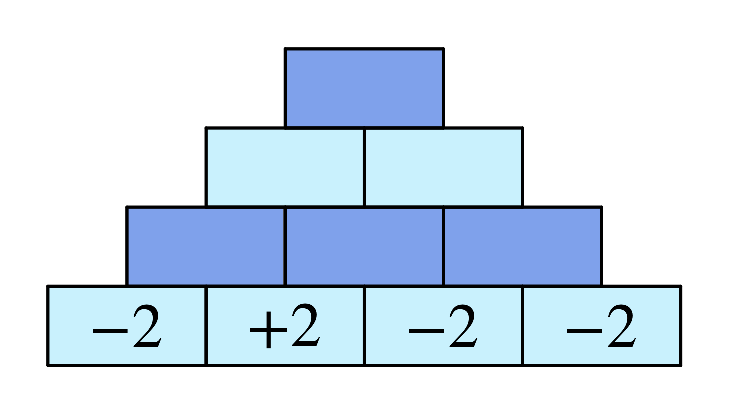
\includegraphics[width=4cm]{pyramide1_MultDivRelatifs} \end{center}
\end{minipage} \hfill%
 \begin{minipage}[c]{0.48\linewidth}
\begin{center} 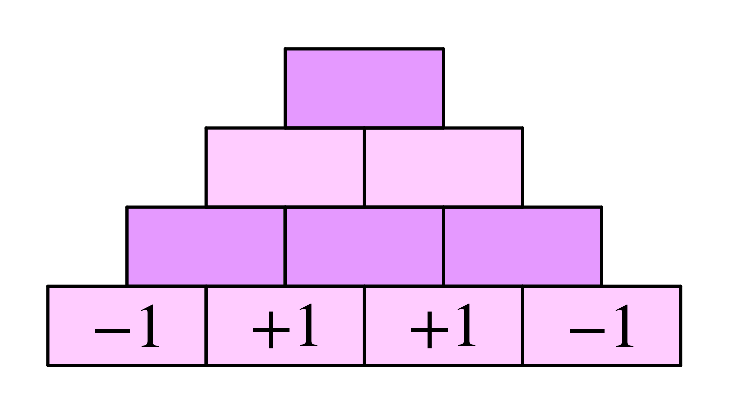
\includegraphics[width=4cm]{pyramide2_MultDivRelatifs} \end{center}  
\end{minipage} \\

\end{exercice}


\begin{exercice}
Donne le signe de chacun des produits suivants :
\begin{enumerate}
 \item $5,4 \times (-3,2) \times (+4) \times (-5,1)$ \ldots \ldots;
 \item $(-0,5) \times (-9) \times 0 \times 7 \times (-1,4) \times (-1)$ \ldots \ldots;
 \item $-6 \times (-10) \times 4 \times (-9) \times (-3) \times (-4,1)$\ldots \ldots.
 \end{enumerate}
\end{exercice}


\begin{exercice}
Effectue les calculs suivants :
\begin{enumerate}
 \item $(-2) \times (-3) \times (+5)$ \dotfill;
 \item $(-3) \times (-2) \times (-4)$  \dotfill;
 \item $(+6) \times (-1) \times (+3)$ \dotfill.
 \end{enumerate}
\end{exercice}


\begin{exercice}
Effectue les calculs suivants :
\begin{enumerate}
 \item $(-3,2) \times (-10) \times (+2) \times (-0,5)$  \dotfill;
 \item $(-75) \times (-0,25) \times (+4) \times (+2)$  \dotfill;
 \item $(-3) \times (-0,1) \times (+5) \times (+4)$  \dotfill;
 \item $(-1,5) \times (+4) \times (-1) \times (+0,8) \times (-3)$  \dotfill;
 \item $(+2) \times (-10) \times (+3) \times (-1) \times (-1)$ \dotfill.
 \end{enumerate}
\end{exercice}


\begin{exercice}
Calcule astucieusement :
\begin{enumerate}
 \item $(-2) \times (-1,25) \times (-2,5) \times (-8)$  \dotfill;
 \item $(-75) \times (-0,25) \times (+2) \times (+4)$  \dotfill;
 \item $(+0,01) \times (-25) \times (-13,2) \times 4 \times (-3)$ \dotfill.
 \end{enumerate}
\end{exercice}


\begin{exercice}
Complète les pointillés par le nombre qui convient :
\begin{colenumerate}{2}
 \item $(-4) \times \ldots = 20$ ;
 \item $(-13) \times \ldots = -39$ ;  
 \item $\ldots \times 7 = -42$ ;
 \item $\ldots \times (-11) = 121$.
 \end{colenumerate}
\end{exercice}


\begin{exercice}
Complète les pointillés par le nombre qui convient :
\begin{colenumerate}{2}
 \item $(+4) \times \ldots = -100$ ;
 \item $(-2,9) \times \ldots = 29$ ;  
 \item $\ldots \times 17 = -17$ ;
 \item $\ldots \times (-3) = -99$.
 \end{colenumerate}
\end{exercice}


\begin{exercice}[Suite logique de nombres]
Donne le signe de chacun des produits suivants :
\begin{enumerate}
 \item $(-1) \times 2 \times (-3) \times 4 \times \ldots \times (-9)$ ;
 \item $(-1) \times (-2) \times (-3) \times (-4) \times \ldots \times (-12)$ ;
 \item $(-4) \times (-3) \times (-2) \times \ldots \times 3 \times 4 \times 5$ ;
 \item $5 \times (-10) \times 15 \times (-20) \times \ldots \times (-100)$ ;
 \item $1 \times (-2) \times 4 \times (-8) \times \ldots \times 1\,024$.
 \end{enumerate}
\end{exercice}


\begin{exercice}[Températures]
Il fait $0^\circ$C et la température chute de deux degrés toutes les heures. 
\begin{enumerate}
 \item Combien de temps faudra-t-il pour que la température atteigne $-10^\circ$C ?
 \item Quelle sera la température dans huit heures ?
 \end{enumerate}
\end{exercice}


\begin{exercice}
Calcule dans chaque cas le produit $x \times y$ :
\begin{colenumerate}{2}
 \item $x = 5$ et $y = -3$ ;
 \item $x = +4$ et $y = -11$ ;
 \item $x = -2$ et $y = -5$ ;
 \item $x = -0,5$ et $y = -5,2$.
 \end{colenumerate}
\end{exercice}


\begin{exercice}
Complète le tableau suivant :
{\small
\begin{center}
\begin{tabular}{|c|c|c|c|c|c|c|}
\hline
\cellcolor{H2} $a$ & \cellcolor{H2} $b$ & \cellcolor{H2} $c$ & \cellcolor{A2} $ab$ &  \cellcolor{A2} ($-a$) $\cdot$ $c$ &  \cellcolor{A2} $-(a\cdot c)$ &  \cellcolor{A2} $a \cdot b \cdot c$ \\\hline 
\cellcolor{H3} $-5$ & \cellcolor{H3} $+6$ & \cellcolor{H3} $-4$ & \cellcolor{A3} & \cellcolor{A3} & \cellcolor{A3} & \cellcolor{A3} \\\hline
\cellcolor{H3} $-1$ & \cellcolor{H3} $-2$ & \cellcolor{H3} $-3$ & \cellcolor{A3} & \cellcolor{A3} & \cellcolor{A3} & \cellcolor{A3} \\\hline
\cellcolor{H3} $-2,1$ & \cellcolor{H3} $-4$ & \cellcolor{H3} $+3$ & \cellcolor{A3} & \cellcolor{A3} & \cellcolor{A3} & \cellcolor{A3} \\\hline
 \end{tabular}
 \end{center}
 } % fin du small
\end{exercice}


\begin{exercice}[Décompositions \ldots]
\begin{enumerate}
 \item Trouve toutes les façons de décomposer le nombre $-20$ en produit de deux nombres entiers relatifs.
 \item Trouve toutes les façons de décomposer le nombre 24 en produit de trois nombres entiers relatifs.
 \end{enumerate}
\end{exercice}


%%%%%%%%%%%%%%%%%%%%%%%%%%%%%%%%%%%
%%%%%%%%%%%%%%%%%%%%%%%%%%%%%%%%%%%
%MiseEnPage
%%%%%%%%%%%%%%%%%%%%%%%%%%%%%%%%%%%
\columnbreak
%%%%%%%%%%%%%%%%%%%%%%%%%%%%%%%%%%%
%%%%%%%%%%%%%%%%%%%%%%%%%%%%%%%%%%%

\begin{exercice}
Sans calculer, donne le signe de chaque résultat :
\begin{colenumerate}{3}
 \item $(-6)^{4}$   \dotfill;
 \item $6^{8}$  \dotfill;
 \item $-132^{51}$  \dotfill;
 \item $(-12)^{15}$  \dotfill;
 \item $(-3)^{7}$  \dotfill;
 \item $(-6)^{100}$  \dotfill;
 \item $-(-35)^{7}$  \dotfill;
 \item $-87^{4}$  \dotfill;
 \item $-(-13^{8})$ \dotfill.
 \end{colenumerate}
\end{exercice}


\begin{exercice}[Puissance de 1 ou de $-1$]
Calcule :
\begin{colenumerate}{4}
 \item $1^{12}$  \dotfill;
 \item $1^{0}$  \dotfill;
 \item $(-1)^{8}$  \dotfill;
 \item $(-1)^{0}$  \dotfill;
 \item $-1^{7}$  \dotfill;
 \item $-1^{6}$  \dotfill;
 \item $(-1)^{9}$  \dotfill;
 \item $-1^{0}$ \dotfill.
 \end{colenumerate}
\end{exercice}

%%%%%%%%%%%%%%%%%%%%%%%%%%%%%%%%%%%%%%%%%%%%%%%%%%%%%%%%%%%%%%%%%%%%%%%%%%%%%

\serie{Quotients de relatifs}

\begin{exercice}
Complète chaque égalité et écris chaque facteur manquant $\lozenge$ sous la forme d'un quotient :
\begin{enumerate}
 \item $(+6) \times \lozenge = +18$ donc $\lozenge = \ldots$ ;
 \item $(+5) \times \lozenge = -20$ donc $\lozenge = \ldots$ ;
 \item $\lozenge \times (-7) = +14$ donc  $\lozenge = \ldots$ ;
 \item $(-2) \times \lozenge = +12$ donc  $\lozenge = \ldots$ ;
 \item $\lozenge \times (-10) = -130$ donc  $\lozenge = \ldots$.
 \end{enumerate}
\end{exercice}


\begin{exercice}
Sans les calculer, donne le signe de chacun des quotients suivants :
\begin{colenumerate}{2}
 \item $(-3) \div (-8)$  \dotfill;
 \item $(+1) \div (-2)$  \dotfill;
 \item $(-4) \div (-5)$  \dotfill;
 \item $(-3,7) \div (+5,1)$ \dotfill.
 \end{colenumerate}
\end{exercice}


\begin{exercice}
Calcule mentalement :
\begin{colenumerate}{2}
 \item $64 \div (-8)$  \dotfill;
 \item $42 \div (-6)$  \dotfill;
 \item $-24 \div (-3)$  \dotfill;
 \item $81 \div (+9)$  \dotfill;
 \item $-17 \div (-1)$  \dotfill;
 \item $-35 \div 7$  \dotfill;
 \item $(-54) \div (-6)$  \dotfill;
 \item $25 \div (-5)$  \dotfill;
 \item $(-4) \div (+4)$  \dotfill;
 \item $(-29) \div (+1)$ \dotfill.
 \end{colenumerate}
\end{exercice}


\begin{exercice}
Calcule mentalement :
\begin{colenumerate}{2}
 \item $(-100) \div (+25)$  \dotfill;
 \item $(-42) \div (-4)$  \dotfill;
 \item $(+54) \div (-3)$  \dotfill;
 \item $(+55) \div (+5)$  \dotfill;
 \item $(-24) \div (-5)$  \dotfill;
 \item $(-13)  \div (-10)$ \dotfill.
 \end{colenumerate}
\end{exercice}


\begin{exercice}
Calcule le quotient de $x$ par $y$ :
\begin{colenumerate}{2}
 \item $x = -15$ et $y = -3$  \dotfill;
 \item $x = +64$ et $y = -8$  \dotfill;
 \item $x = -36$ et $y = 12$  \dotfill;
 \item $x = -2,4$ et $y = 1,2$  \dotfill;
 \item $x = y = -2,3$  \dotfill;
 \item $x = 0$ et $y = -5$ \dotfill.
 \end{colenumerate}
\end{exercice}


\begin{exercice}
Complète le tableau suivant et donne le résultat sous forme décimale :
{\small
\begin{center}
\begin{tabular}{|c|c|c|c|c|c|}
\hline
\cellcolor{H2} $a$ & \cellcolor{H2} $b$ & \cellcolor{H2} $c$ & \cellcolor{A2} $a : b$ & \cellcolor{A2} $(-b) : c$ & \cellcolor{A2} $c : (-a)$ \\\hline 
\cellcolor{H3} $-5$ & \cellcolor{H3} $+4$ & \cellcolor{H3} $-4$ & \cellcolor{A3} & \cellcolor{A3} & \cellcolor{A3} \\\hline
\cellcolor{H3} $-2,5$ & \cellcolor{H3} $-1$ & \cellcolor{H3} $+20$ & \cellcolor{A3} & \cellcolor{A3} & \cellcolor{A3} \\\hline
\cellcolor{H3} $+8$ & \cellcolor{H3} $-4$ & \cellcolor{H3} $-0,5$ & \cellcolor{A3} & \cellcolor{A3} & \cellcolor{A3} \\\hline
\cellcolor{H3} $-2,4$ & \cellcolor{H3} $-1,2$ & \cellcolor{H3} $-24$ & \cellcolor{A3} & \cellcolor{A3} & \cellcolor{A3} \\\hline
 \end{tabular}
 \end{center}
 } % fin du small
\end{exercice}


\begin{exercice}
Donne, à l'aide de ta calculatrice, l'arrondi à l'unité de chacun des nombres suivants, comme dans l'exemple : \\[0.5em]
Exemple : $A = \dfrac{-153}{23}$. \\[0.5em]
La calculatrice donne $A \approx -6,652173913$. \\[0.5em]
On a donc : $-7 < A < -6$. \\[0.5em]
L'arrondi à l'unité de $A$ est $-7$ car $A$ est plus proche de $-7$ que de $-6$.
\begin{colitemize}{3}
 \item $B = \dfrac{39}{-9}$ ;
 \item $C = \dfrac{-17}{-7}$ ;
 \item $D = \dfrac{-28}{51}$.
 \end{colitemize}
\end{exercice}

%%%%%%%%%%%%%%%%%%%%%%%%%%%%%%%%%%%%%%%%%%%%%%%%%%%%%%%%%%%%%%%%%%%%%%%%%%%%%

\serie{Calculs variés}

\begin{exercice}
Pour chacun des calculs suivants, indique s'il s'agit d'une somme ou d'un produit, puis donne le résultat :
\begin{colenumerate}{2}
 \item $-4 \times (+9)$ ;
 \item $-3 - (+8)$ ;
 \item $-7 + (-5)$ ;
 \item $3 \times (-7)$ ;
 \item $-8 + (+6)$ ;
 \item $+9 \times (+3)$ ;
 \item $-5 - (-16)$ ;
 \item $-11 \times (-4)$.
 \end{colenumerate}
\end{exercice}


\begin{exercice}
Sans calculer, donne le signe de chaque résultat :
\begin{colenumerate}{2}
 \item $(-4) \times (-12)$  \dotfill;
 \item $(+15) + (-22)$  \dotfill;
 \item $(-45) - (-51)$  \dotfill;
 \item $(-37) \times (+51)$  \dotfill;
 \item $(+7) \times (+8)$  \dotfill;
 \item $(-7) + (+8)$  \dotfill;
 \item $(-3,12) \times (-2,5)$  \dotfill;
 \item $(-3,17) - (+3,7)$ \dotfill.
 \end{colenumerate}
\end{exercice}


\begin{exercice}
Calcule mentalement :
\begin{colenumerate}{2}
 \item $8 \times (-8)$  \dotfill;
 \item $-22 + (-6)$  \dotfill;
 \item $-14 \times 3$  \dotfill;
 \item $-5 - (+17)$  \dotfill;
 \item $(-34) + (-19)$  \dotfill;
 \item $-15 \times (-5)$ \dotfill.
 \end{colenumerate}
\end{exercice}


\begin{exercice}
Calcule mentalement :
\begin{colenumerate}{2}
 \item $(-4) \times (-2,5)$  \dotfill;
 \item $(+3,5) + (-2,2)$  \dotfill;
 \item $(-3,9) + (-5,4)$  \dotfill;
 \item $(-3) \times (+4,2)$  \dotfill;
 \item $(+2,6) \times (-3)$  \dotfill;
 \item $(-7,15) - (-2,2)$  \dotfill;
 \item $(-3,12) \times (-10)$  \dotfill;
 \item $(-0,7) - (+1,17)$ \dotfill.
 \end{colenumerate}
\end{exercice}


\begin{exercice}
Remplace les pointillés par le signe opératoire qui convient :
\begin{colenumerate}{2}
 \item $(-3) \ldots (-2) = -5$ ;
 \item $(-3) \ldots (-2) = +6$ ;
 \item $(-2) \ldots (-2) = +4$ ;
 \item $(-2) \ldots (-2) = -4$ ;
 \end{colenumerate}
\begin{enumerate}
\setcounter{enumi}{4}
\vspace{-1.5em}
\item $(-5) \ldots (+4) = (-12) \ldots (+8)$.
\end{enumerate}
 \end{exercice}

 
 %%%%%%%%%%%%%%%%%%%%%%%%%%%%%%%%%%%
%%%%%%%%%%%%%%%%%%%%%%%%%%%%%%%%%%%
%MiseEnPage
%%%%%%%%%%%%%%%%%%%%%%%%%%%%%%%%%%%
\columnbreak
%%%%%%%%%%%%%%%%%%%%%%%%%%%%%%%%%%%
%%%%%%%%%%%%%%%%%%%%%%%%%%%%%%%%%%%

\begin{exercice}[Logique !]
Complète chaque suite de nombres :
\begin{enumerate}
 \item 3 ; 1 ; $-1$ ; \ldots  \ldots; \ldots  \ldots; \ldots  \ldots;
 \item 1 ; $-2$ ; $+4$ ; \ldots  \ldots; \ldots  \ldots; \ldots  \ldots;
 \item $-16$ ; 8 ; $-4$ ; \ldots  \ldots; \ldots  \ldots; \ldots \ldots ;
 \item 0,5 ; $- 5$ ; 50 ; \ldots  \ldots; \ldots  \ldots; \ldots \ldots .
 \end{enumerate}
\end{exercice}


\begin{exercice}
Complète les « pyramides » sachant que le nombre contenu dans une case est le produit des nombres contenus dans les deux cases situées en dessous de lui : \\[0.3em]

\begin{minipage}[c]{0.48\linewidth}
\begin{center} 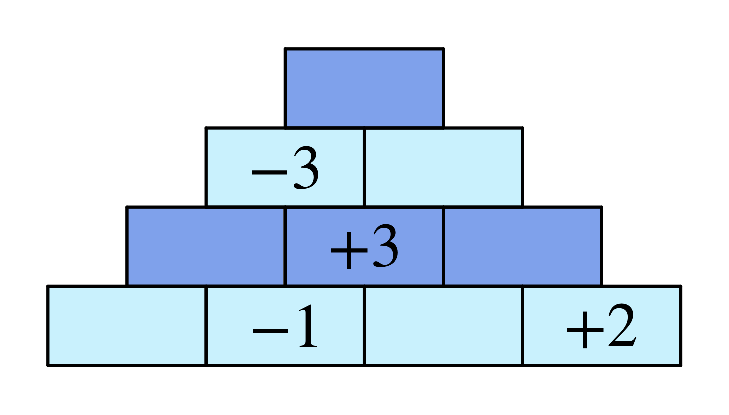
\includegraphics[width=4cm]{pyramide3_MultDivRelatifs} \end{center}
\end{minipage} \hfill%
 \begin{minipage}[c]{0.48\linewidth}
\begin{center} 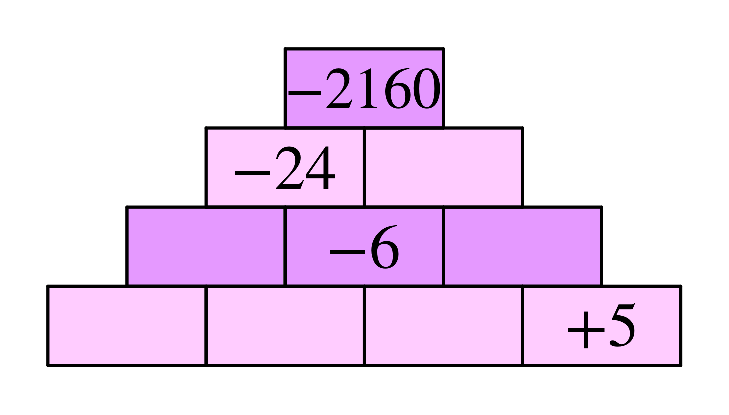
\includegraphics[width=4cm]{pyramide4_MultDivRelatifs} \end{center}  
\end{minipage} \\
\end{exercice}


\begin{exercice}
Effectue les calculs suivants en détail :
\begin{colenumerate}{2}
 \item $7 + (-6) \times (-6)$ ;
 \item $13 - (+3) \times (-4) - 8$ ;
 \item $-30 : (-9 + 15)$ ;
 \item $-3 -9 \times (-3)$ ;
 \item $-3 \times 6 \times (-2 + 8)$.
 \end{colenumerate}
\end{exercice}


\begin{exercice}
Effectue les calculs suivants en détail :
{\footnotesize
\begin{colenumerate}{2}
 \item $-22 + (13 - 5) \times (-5)$;
 \item $(-2) \times 8 + 2 \times (-20) : 4$;
 \item $-28 + (5 - 2) \times (-4)$;
 \item $7 \times (-7) + 3 \times (-25) : (-5)$;
 \item $3,2 \times (-6) + (-2,3 - 7,7)$;
 \item $150 : (-1,2 - 9 \times 3,2)$.
 \end{colenumerate}}
\end{exercice}


\begin{exercice}[Vocabulaire]
\begin{enumerate}
 \item Traduis les phrases suivantes par un calcul :
 \begin{itemize}
  \item \textcolor{A1}{La somme du produit de 4 par $-5$ et de $-6$ ;}
  \item \textcolor{H1}{Le produit de la somme de 7 et de $-8$ par la somme de 8 et de $-2$.}
  \end{itemize}  
 \item Effectue ces calculs.
 \end{enumerate}
\end{exercice}


\begin{exercice}[Vocabulaire (bis)]
Traduis les expressions mathématiques suivantes par des phrases. \\[0.2em]
Exemple : $(-2) \times 3 + 1$ se traduit par \\[0.2em]
« \textcolor{A1}{La somme du produit de $(-2)$ par 3 et de 1.} »\\
{\small
\begin{colenumerate}{2}
 \item $A = 5 \times (-7) + 3$ ;
 \item $B = 3 + 2 : (-4)$ ;
 \item $C = 7 - 4 \times (-10)$ ;
 \item $D = (2 - 3) \times (-1 - 2)$ ;
 \item $E = (1 - 7) : (2 + 5)$ ;
 \item $F = -2 +(-6) \times (6) - 9$.
 \end{colenumerate}}
\end{exercice}


\begin{exercice}
Complète le tableau suivant :
{\small
\begin{center}
\begin{tabular}{|c|c|c|c|c|c|c|}
\hline
\cellcolor{H2} $a$ & \cellcolor{H2} $b$ & \cellcolor{H2} $c$ & \cellcolor{A2} $a$ $\times$ $b$ &  \cellcolor{A2} ($-$ $a$) $\times$ $c$ &  \cellcolor{A2} $-$ ($a$ $\times$ $c$) &  \cellcolor{A2} $a$ $\times$ $b$ $\times$ $c$ \\\hline 
\cellcolor{H3} $-5$ & \cellcolor{H3} & \cellcolor{H3} $+4$ & \cellcolor{A3} & \cellcolor{A3} & \cellcolor{A3} & \cellcolor{A3} \\\hline
\cellcolor{H3} & \cellcolor{H3} & \cellcolor{H3} $+2$ & \cellcolor{A3} & \cellcolor{A3} & \cellcolor{A3} $-12$ & \cellcolor{A3} $-36$ \\\hline
 \end{tabular}
 \end{center}
 } % fin du small
\end{exercice}
